\documentclass[tikz]{standalone}
\usepackage{amsmath}
\usepackage{xcolor}
\definecolor{bg}{HTML}{171D2B}
\definecolor{aksen}{HTML}{F7B538}
\definecolor{biru}{HTML}{60A5FA}
\definecolor{hijau}{HTML}{34D399}
\pagecolor{bg}
\begin{document}
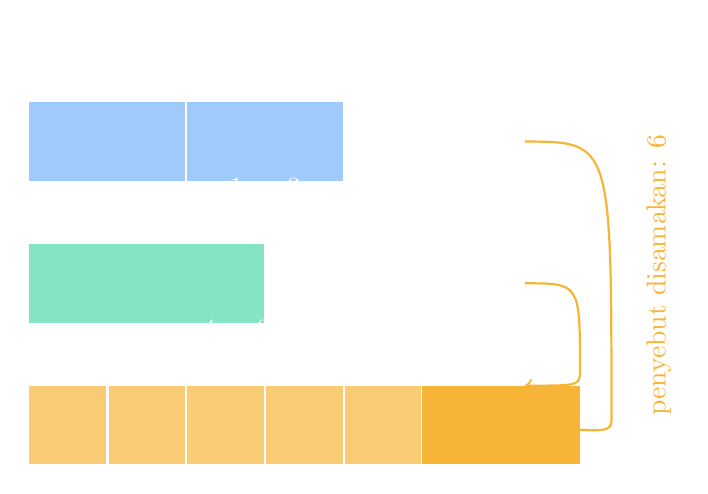
\begin{tikzpicture}[x=1cm,y=1cm]
% --- bar 2/3 ---
\draw[white,thick] (0,3) rectangle (6,4);
\fill[biru!60] (0,3) rectangle (4,4);
\draw[white,thick] (2,3) -- (2,4);
\draw[white,thick] (4,3) -- (4,4);
\node[white,above] at (3,4) {$\dfrac{2}{3} = \dfrac{4}{6}$};
% --- bar 1/2 ---
\draw[white,thick] (0,1.2) rectangle (6,2.2);
\fill[hijau!60] (0,1.2) rectangle (3,2.2);
\draw[white,thick] (3,1.2) -- (3,2.2);
\node[white,above] at (3,2.2) {$\dfrac{1}{2} = \dfrac{3}{6}$};
% --- hasil ---
\draw[white,thick] (0,-0.6) rectangle (7,0.4);
\fill[aksen!70] (0,-0.6) rectangle (7,0.4);
\foreach \i in {1,...,6} \draw[white,thick] (\i, -0.6) -- (\i, 0.4);
\fill[aksen] (5,-0.6) rectangle (7,0.4);
\node[white,above] at (3,0.4) {$\dfrac{4}{6} + \dfrac{3}{6} = \dfrac{7}{6}$};
% --- panah penyebut ---
\draw[aksen,thick,->] (6.3,3.5) .. controls (7.4,3.5) .. (7.4,0) .. controls (7.4,-0.2) .. (6.3,-0.1);
\draw[aksen,thick,->] (6.3,1.7) .. controls (7.0,1.7) .. (7.0,0.6) .. controls (7.0,0.4) .. (6.3,0.4);
\node[aksen,rotate=90] at (8.0,1.8) {penyebut disamakan: 6};
\end{tikzpicture}
\end{document}
